\lecture{4}{2026-09-16}{}

% Simple closed form -> Taylor series -> asymptotics
% Sum of simple terms -> integration -> asymptotics

\begin{theorem}
    Let \(a < b\) be integers.
    Let \(f\) be continuous on \([a-1, b+1]\).
    If \(f\) is increasing on \([a-1, b+1]\), then
    \[
        \int_{a-1}^{b} f(x) \, dx \le \sum_{k=a}^{b} f(k) \le \int_{a}^{b+1} f(x) \, dx.
    \]
    If \(f\) is decreasing on \([a-1, b+1]\), then
    \[
        \int_{a}^{b+1} f(x) \, dx \le \sum_{k=a}^{b} f(k) \le \int_{a-1}^{b} f(x) \, dx.
    \]
\end{theorem}

\begin{corollary}
    If \(f\) is monotone on \([a-1, b+1]\) and \(|f(x)| \le M\) on \([a-1, b+1]\), then
    \[
        \left| \sum_{k=a}^{b} f(k) - \int_{a}^{b} f(x) \, dx \right| \le M.
    \]
\end{corollary}

\begin{proof}
    \[
        -M \leq \int_{a-1}^{a} f(x) \, dx \leq \sum_{k=a}^{b} f(k) - \int_{a}^{b} f(x) \, dx \leq \int_{b}^{b+1} f(x) \, dx \leq M.
    \]
\end{proof}

\section*{Euler--Maclaurin summation formula}

The Bernoulli numbers \(B_k\) are defined by the generating function
\[
    \frac{t}{e^t - 1} = \sum_{k=0}^{\infty} B_k \frac{t^k}{k!}.
\]

\begin{theorem}
Suppose \(f\) is \(m\)-times continuously differentiable on \([a-1, b+1]\).
Then
\[
    \sum_{k=a}^{b} f(k)
    = \int_{a}^{b} f(x) \, dx 
    + \sum_{k=1}^m \frac{B_k}{k!} \left( f^{(k-1)}(b) - f^{(k-1)}(a) \right)
    + R_m,
\]
where the remainder term \(R_m\) satisfies
\[
    |R_m| \leq \frac{2 \zeta(m)}{(2\pi)^m} \int_{a-1}^{b+1} |f^{(m)}(x)| \, dx,
\]
and \(\zeta(m)\) is the Riemann zeta function.
\end{theorem}

The proof is not enlightening.

\begin{example}
    Let \(f(x) = x^2\). We figured out before that \(\sum_{k=0}^{n} k^2 = \frac{n^3}{3} + O(n^2)\).
    Using the Euler--Maclaurin formula with \(m=3\), we have
    \[
        \sum_{k=0}^{n} k^2 = \int_0^n x^2 \, dx + \frac{B_1}{1!} (f(n) - f(0)) + \frac{B_2}{2!} (f'(n) - f'(0)) + \frac{B_3}{3!} (f''(n) - f''(0)) + R_3.
    \]
    The remainder term \(R_3\) satisfies
    \[
        |R_3| \leq \frac{2 \zeta(3)}{(2\pi)^3} \int_{-1}^{n+1} |f^{(3)}(x)| \, dx = 0,
    \]
    since \(f^{(3)}(x) = 0\).
    Therefore, we have
    \[
        \sum_{k=0}^{n} k^2 = \frac{n^3}{3} + \frac{n^2}{2} + \frac{n}{6} = \frac{n(n+1)(2n+1)}{6}.
    \]
\end{example}

This is the classical techniques that solves stuff for the easier cases.
We're not gonna use them much, but it's a good thing to know because the later stuff will be basically studying things where this more classical technique doesn't work.

\section*{Analytic Combinatorics}

Everything from now on is on \cite{Melczer2021}.

We'll focus on asymptotics directly from generating functions, not from closed forms or sums.

For this, we need complex analysis.

We can write \(z = a + bi = r e^{i\theta}\) where \(r = |z| = \sqrt{a^2 + b^2}\) and \(\theta = \arg(z)\) defined up to an integer multiple of \(2\pi\).

You need \(\mathbb{C}\) to study series and generating functions properly.

\begin{example}
    The series expansion
    \[
    \frac{1}{1-z} = \sum_{n \ge 0} z^n
    \]
    converges for \(|z| < 1\).

    The series expansion
    \[
    \frac{1}{1+z^2} = \sum_{n \ge 0} (-1)^n z^{2n}
    \]
    converges for \(|z| < 1\).
\end{example}

Our presentation is centered around series.

An \emph{open disk} centered at \(a \in \mathbb{C}\) of radius \(r > 0\) is the set
\[
    D_a^{(r)} = \{ z \in \mathbb{C} : |z - a| < r \}.
\]

\begin{figure}
    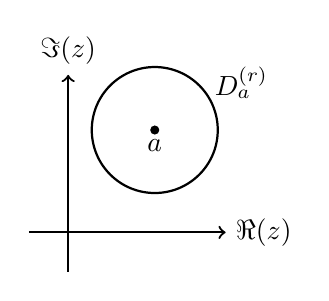
\begin{tikzpicture}
        \draw[thick,->] (-.5,0) -- (2,0) node[right] {$\Re(z)$};
        \draw[thick,->] (0,-.5) -- (0,2) node[above] {$\Im(z)$};
        \coordinate (center) at (1.1, 1.3);
        \draw[fill=black] (center) circle (.05);
        \node[below] at (center) {$a$};
        \draw[thick] (center) circle (.8);
        \node at (2.2, 1.9) {$D_a^{(r)}$};
    \end{tikzpicture}
\end{figure}

A set \(O \in \mathbb{C}\) is \emph{open} if for every \(a \in O\), there exists \(r > 0\) such that \(D_a^{(r)} \subseteq O\).

A connected open set is called a \emph{domain}.
A \emph{neighborhood} of \(a \in \mathbb{C}\) is an open set containing \(a\).

A function \(f(z)\) is \emph{analytic} at \(z = a\) if there exists a neighborhood \(N\) of \(a\) such that \(f(z)\) is representable by a convergent power series
\[
    f(z) = \sum_{n=0}^{\infty} c_n (z - a)^n
\]
for all \(z \in N\).
A function \(f(z)\) is \emph{analytic} on a domain \(\Omega\) if it is analytic at every point of \(\Omega\).

\begin{example}
    The function \(f(z) = \frac{1}{1-z}\) has the representation \(f(z) = \sum_{n \ge 0} z^n\) for \(|z| < 1\), so it is analytic on the open disk \(D_0^{(1)}\), so \(f\) is analytic on \(D_0^{(1)}\).

    Note that
    \[
        f(z) = \frac{1/2}{1 - \frac{z + 1}{2}} = \frac{1}{2} \sum_{n \ge 0} 2^{-n} (z + 1)^n,
    \]
    so \(f\) is also analytic on the open disk \(D_{-1}^{(2)}\).
\end{example}

\begin{proposition}
    If \(f\) is analytic on a domain \(\Omega\), then
    \[
        f'(a) = \lim_{z \to a} \frac{f(z) - f(a)}{z - a}
    \]
    exists for all \(a \in \Omega\).
    The derivative satisfies the usual sum, product, chain rules, etc.
\end{proposition}

\begin{proposition}
    If \(f\) is analytic and \(f(x + iy) = a(x, y) + i b(x, y)\), then \(a\) and \(b\) satisfy the Cauchy--Riemann equations
    \[
        \frac{\partial a}{\partial x} = \frac{\partial b}{\partial y} \quad \text{and} \quad \frac{\partial a}{\partial y} = -\frac{\partial b}{\partial x}.
    \]
\end{proposition}

\begin{proposition}
    If \(f\) and \(g\) are analytic on a domain \(\Omega\) and agree on a non-empty open subset of \(\Omega\), then \(f = g\) on all of \(\Omega\).
\end{proposition}